\begin{document}
	
	\section{Pipeline Description}
	
	As I've said before the aim of these thesis is the developing of a pipeline for the identification of GGO and CS areas in chest CT scans of COVID-19 affected patients. The pipeline aims to have the following characteristics:   
	\begin{itemize}
		\item  \textbf{Fully Automated: } to remove the dependency from an external operator, and so the subjectivity of the segmentation; 
		
		\item \textbf{Fast: } in order to compete with certified software and to provides a segmentation in few minutes.
	\end{itemize}

	The pipeline is unsupervised, so doesn't requires to provide the expected outcomes, so the labels where used only for the quality check. During the pipeline developing we have to takes into account is that the infection regions may have different patterns according to the stage of the disease or recovery, as we can see in \figurename\,\ref{fig:GGO-Spatial}, and usually these patterns are spatially disconnected; so we have decided to use a pixel classification technique.
	
	%To develop the pipeline I've work mainly on 83 anonymized CT scans of patients affected by COVID-19 kindly provided by Sant'Orsola hospital. For each of these scans was also provided a segmentation made by internals. As a benchmark I've also used ZENODO~\cite{DATA:ZENODO} and MOSMED~\cite{DATA:MOSMED}, which are two public available data set, described in details in Chapter 2.\\
	%Even if 3 data set are available, the amount of data isn't high, that because COVID-19 is a new disease. Moreover the available manual segmentation aren't always goods, some of them presents some errors and misclassified areas.\\
	%The low number of scans and the quality of labels have discouraged the use of supervised segmentation techniques like classifiers or neural networks.\\
	%In the end a completely unsupervised technique was used, which doesn't requires to provides already segmented images as prior knowledge.\\
	%An other thing to takes into account during the developing, is that the lesions may have different patterns according to the stage of the disease or the patients as in \figurename\,\ref{fig:GGO-Spatial} and usually these patterns are spatially disconnected, so to perform the segmentation a pixel classification techniques was used.
	
	\begin{figure}[h!]
		\centering
			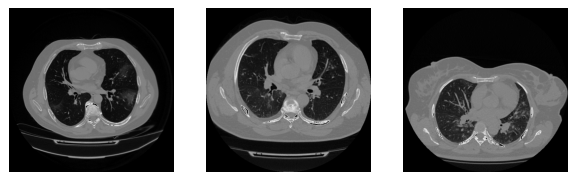
\includegraphics[scale=1.5]{GGOSeveralPatients.png}
		\caption{Groud Glass Opacity of COVID-19 affected patients with different severity of the disease. From left to right this scans belong to CT-1, CT-2 and CT-4 category of MOSMED~\cite{DATA:MOSMED} dataset}
	\label{fig:GGO-Spatial}
	\end{figure}
	
	In the end the basic idea was to use the Color Quantization as medical imaging segmentation , which aims to to identify the different type of tissue and lesions by grouping them by color similarity. In particular we aims to assign to each structure inside the lung a characteristic colors and label each voxel by identify it as belonging to the tissue with the most similar characteristic color. This approach is justified since exist a relation between the kind of tissue and the color used to display it in a CT scan, given by Hounsfield Unit.\\
	Since it is unlikely to find a structure with a single voxel extension, I've used the multi-channel characteristics of digital images to takes into accounts also the neighboring voxels.\\
	
	In this section I will describe how color quantization works for image segmentation, how the color space was build in order to incorporate also neighboring information and the final structure of the segmentation pipeline.

\end{document}